\documentclass[11pt, dvipsnames, handout]{beamer}
\newtoggle{full}
\settoggle{full}{true}

\newtoggle{covered}
\settoggle{covered}{false}

\newtoggle{presentable}
\settoggle{presentable}{false}

\newtoggle{dualscreen}
\settoggle{dualscreen}{false}

\usepackage{pgfplots}
%\pgfplotsset{compat = newest}

\usepackage{pgfpages}

\setbeamertemplate{note page}{\pagecolor{yellow!5}\vfill \insertnote \vfill}
\usepackage{collect}
\definecollection{notes}
\newcounter{notestaken}

\usepackage{xpatch}

\usepackage{ulem}

\usepackage[framemethod=tikz]{mdframed}

\usepackage{scalerel}
\usepackage{calc}

%\usepackage{enumitem}
\setlength\fboxsep{.2em}

\usepackage{graphicx} % Allows including images
\usepackage{booktabs} % Allows the use of \toprule, \midrule and \bottomrule in tables

\xpatchcmd{\itemize}
  {\def\makelabel}
  {\setlength{\itemsep}{0.65 em}\def\makelabel}
  {}
  {}


\xpatchcmd{\beamer@enum@}
  {\def\makelabel}
  {\setlength{\itemsep}{0.65 em}\def\makelabel}
  {}
  {}


%\makeatletter
%\renewcommand{\itemize}[1][]{%
%  \beamer@ifempty{#1}{}{\def\beamer@defaultospec{#1}}%
%  \ifnum \@itemdepth >2\relax\@toodeep\else
%    \advance\@itemdepth\@ne
%    \beamer@computepref\@itemdepth% sets \beameritemnestingprefix
%    \usebeamerfont{itemize/enumerate \beameritemnestingprefix body}%
%    \usebeamercolor[fg]{itemize/enumerate \beameritemnestingprefix body}%
%    \usebeamertemplate{itemize/enumerate \beameritemnestingprefix body begin}%
%    \list
%      {\usebeamertemplate{itemize \beameritemnestingprefix item}}
%      {%
%        \setlength\topsep{1em}%NEW
%        \setlength\partopsep{1em}%NEW
%        \setlength\itemsep{1em}%NEW
%        \def\makelabel##1{%
%          {%
%            \hss\llap{{%
%                \usebeamerfont*{itemize \beameritemnestingprefix item}%
%                \usebeamercolor[fg]{itemize \beameritemnestingprefix item}##1}}%
%          }%
%        }%
%      }
%  \fi%
%  \beamer@cramped%
%  \raggedright%
%  \beamer@firstlineitemizeunskip%
%}
%
%
%
%
%
%\makeatother

%\setlist[beamer@enum@]{topsep=1 em}
%\let\origcheckmark\checkmark %screw you dingbat
%\let\checkmark\undefined %screw you dingbat
%\usepackage{dingbat} 
%\let\checkmark\origcheckmark %screw you dingbat






%\usepackage{fontawesome}

\usepackage{mathtools}
\usepackage{etoolbox, calculator}

\usepackage{xcolor}
\usepackage{tikz}
\usetikzlibrary{arrows.meta}
\usetikzlibrary{calc}
\usepackage[nomessages]{fp}
\usepackage{transparent}
\usepackage{accsupp}
%\usepackage{color, xcolor}

%colorblind-friendly palette
%\definecolor{dblue}{RGB}{51,34,136}
\definecolor{lblue}{RGB}{136,204,238}
%\definecolor{green}{RGB}{17,119,51}
\definecolor{tan}{RGB}{221,204,119}
%\definecolor{mauve}{RGB}{204,102,119}

\usepackage{tcolorbox}



\usepackage{xifthen}
\usepackage{nicefrac}
\usepackage{amsmath}
\usepackage{amsthm}
\usepackage{amssymb}
\theoremstyle{definition}
\newtheorem*{define}{Definition}
\newtheorem*{recall}{Recall}


\DeclareMathOperator{\tr}{tr}

\usepackage{multicol}
%\setlength{\columnsep}{1cm}

\usepackage{tablists, amsmath,vwcol, cancel, polynom}
\usetikzlibrary{shapes, patterns, decorations.shapes}
%\usepackage{tikzpeople}
\tikzstyle{vertex}=[shape=circle, minimum size=2mm, inner sep=0, fill]
\tikzstyle{opendot}=[shape=circle, minimum size=2mm, inner sep=0, fill=white, draw]

% common math quick commands
\newcommand{\nicedd}[2]{\nicefrac{\text{d}#1}{\text{d}#2}}
\newcommand{\dd}[2]{\dfrac{\text{d}#1}{\text{d}#2}}
\newcommand{\pd}[2]{\dfrac{\partial #1}{\partial#2}}
\renewcommand{\d}[1]{\text{d}#1}
\newcommand{\ddn}[3]{\dfrac{\text{d}^{#3}#1}{\text{d}#2^{#3}}}
\newcommand{\pdn}[3]{\dfrac{\partial^{#3}#1}{\partial#2^{#3}}}
\newcommand{\p}[0]{^{\prime}}
\newcommand{\pp}[0]{^{\prime\prime}}
\newcommand{\op}[2][\text{L}]{#1 \left[ #2 \right]}

\newcommand{\lap}[1]{\mathcal{L}\left\{#1\right\}}
\newcommand{\lapinv}[1]{\mathcal{L}^{-1}\left\{#1\right\}}
\newcommand{\lapint}[1]{\int_0^\infty e^{-st}#1dt}
\newcommand{\evalat}[2]{\Big|_{#1}^{#2}}

\newcommand{\paren}[1]{ \left( #1 \right)}

\newcommand{\haxis}[4][\normcolor]{\draw[#1, <->] (-#2,0)--(#3,0) node[right]{$#4$}; }

\newcommand{\circled}[1]{\raisebox{.5pt}{\textcircled{\raisebox{-.9pt} {#1}}}}
\newcommand{\axis}[4]{\draw[\normcolor, <->] (-#1,0)--(#2,0) 
node[right]{$x$};
\draw[help lines, <->] (0,-#3)--(0,#4) node[above]{$y$};}

\newcommand{\laxis}[6]{\draw[<->] (-#1,0)--(#2,0) 
node[right]{$#5$};
\draw[ <->] (0,-#3)--(0,#4) node[above]{$#6$};}
\newcommand{\xcoord}[2]{
	\draw (#1,.2)--(#1,-.2) node[below]{$#2$};}
\newcommand{\textnode}[3]{
	\draw (#1,#2) node[below]{$#3$};}
	
\newcommand{\nxcoord}[2]{
	\draw (#1,-.2)--(#1,.2) node[above]{$#2$};}
\newcommand{\ycoord}[2]{
	\draw (.2,#1)--(-.2,#1) node[left]{$#2$};}
\newcommand{\nycoord}[2]{
	\draw (-.2,#1)--(.2,#1) node[right]{$#2$};}
\newcommand{\dlim}{\displaystyle\lim}
\newcommand{\dlimx}[1]{\displaystyle\lim_{x \rightarrow #1}}
\newcommand{\stickfig}[2]{
	\draw (#1,#2) arc(-90:270:2mm);
	\draw (#1,#2)--(#1,#2-.5) (#1-.25,#2-.75)--(#1,#2-.5)--(#1+.25,#2-.75) (#1-.2,#2-.2)--(#1+.2,#2-.2);}	

%\newcounter{example}
%\setcounter{example}{1}
%\newcounter{preFrameExample}
%\AtBeginEnvironment{frame}{\setcounter{preFrameExample}{\value{example}}}
%\newcommand{\ex}[1]{
%	 \setcounter{example}{\value{preFrameExample}}
%	 \textcolor{green}{\small\fbox{Example \arabic{example}: #1}}\\[8pt]
%	\stepcounter{example}}
%\newcommand{\exans}[1]{
%	\SUBTRACT{\value{preFrameExample}}{1}{\n}
%	 \textcolor{green}{\small\fbox{Solution \n: #1}}\\[8pt]}
\mode<presentation> {

% The Beamer class comes with a number of default slide themes
% which change the colors and layouts of slides. Below this is a list
% of all the themes, uncomment each in turn to see what they look like.


\usetheme{CambridgeUS}
\usecolortheme[named=black]{structure}


\newcommand{\studentcolor}[0]{ForestGreen}
\newcommand{\normcolor}[0]{NavyBlue}
\newcommand{\alertcolor}{Red}

\setbeamercolor{normal text}{fg=\normcolor}
\setbeamercolor{frametitle}{fg=\normcolor}
\setbeamercolor{section in head/foot}{fg=Black, bg=Gray!20}
\setbeamercolor{subsection in head/foot}{fg=Green!70!Black, bg=Gray!10}
\setbeamercolor{alerted text}{fg=\alertcolor}
\setbeamerfont{alerted text}{series=\bf}
\setbeamertemplate{enumerate items}[default]
\setbeamercolor{enumerate item}{fg=\normcolor}

\setbeamertemplate{footline} % To remove the footer line in all slides uncomment this line
%\setbeamertemplate{footline}[page number] % To replace the footer line in all slides with a simple slide count uncomment this line

\setbeamertemplate{navigation symbols}{} % To remove the navigation symbols from the bottom of all slides uncomment this line
}

\newcommand{\alertbox}[1]{\tcbox[on line, colframe=\alertcolor, colback=White, left=2pt,right=2pt,top=2pt,bottom=2pt]{\usebeamercolor*{normal text}#1}}


\newcommand{\startstu}{\setbeamercolor{normal text}{fg=\studentcolor}\usebeamercolor*{normal text}\setbeamercolor{enumerate item}{fg=\studentcolor}\usebeamercolor*{enumerate item}}
\newcommand{\stopstu}{\setbeamercolor{normal text}{fg=\normcolor}\usebeamercolor*{normal text}\setbeamercolor{enumerate item}{fg=\normcolor}\usebeamercolor*{enumerate item}}

\newcommand{\takenote}[1]{ \begin{collect}{notes}{}{}{}{}  #1  \end{collect}  \addtocounter{notestaken}{1}} %\ifthenelse{\value{notestaken}>0}{\hrulefill\\}{}

\makeatletter
\newcommand{\cover}{\alt{\beamer@makecovered}{\beamer@fakeinvisible}}
\newcommand{\ucover}[1]{\iftoggle{full}{}{\beamer@endcovered} \stopstu #1\startstu \iftoggle{full}{}{\beamer@startcovered} }
%\newcommand{\ucover}[1]{\beamer@endcovered \stopstu #1\startstu \beamer@startcovered }
\makeatother

\newcommand{\skippause}{ \addtocounter{beamerpauses}{-1}}
\newcommand{\blockpres}{ \skippause \pause }

\newcommand{\studentify}[1]{\startstu #1  \stopstu }
\newcommand{\student}[1]{\iftoggle{full}{ \pause  \studentify{#1} }{\iftoggle{covered}{\studentify{#1}}{\cover{  #1 }}}}
\newcommand{\cstudent}[1]{\student{\begin{center} #1 \end{center}}}
\newcommand{\fullonly}[1]{\iftoggle{full}{ #1}{}}
\newcommand{\presentonly}[1]{\iftoggle{presentable}{ #1}{}}

\usepackage{xparse}
\usepackage{xifthen}

% shortcuts for commonly-used presentation elements
%\NewDocumentCommand{\slide}{o m}
% {\IfValueTF{#1}{\begin{frame}[t]{#1}}{\begin{frame}[t]} #2 \end{frame}}

\newtoggle{iscovered}

\newcommand{\slide}[2][]{%
%\setcounter{notestaken}{0}
\takenote{#2} 
%\ifthenelse{\equal{#1}{}}{\begin{frame}[t]}{\begin{frame}[t]{#1}} #2 \ifthenelse{\value{notestaken}>0}{ \note{\includecollection{notes}}}{} \end{frame}%
\ifthenelse{\equal{#1}{}}{\begin{frame}[t]}{\begin{frame}[t]{#1}} #2 \iftoggle{covered}{\settoggle{iscovered}{true}}{\settoggle{iscovered}{false}}  \note{ \iftoggle{iscovered}{}{\settoggle{covered}{true}} #2 \iftoggle{iscovered}{}{\settoggle{covered}{false}} } \end{frame}%
%\setcounter{notestaken}{0}
}
\newcommand{\defn}[2][]{%
 \setcounter{listcounter}{0}%
\ifthenelse{\equal{#1}{}}{\begin{block}{Definition}}{\begin{block}{#1 :}}%
 #2 \vspace{0.25em} \ifthenelse{\value{listcounter}>0}{\skippause}{} \pause \end{block}%
}



\newcommand{\arr}[2]{\begin{array}{#1}#2\end{array}}
\newcommand{\mat}[2]{\left[\arr{#1}{#2}\right]}
\newcommand{\carray}[1]{\arr{c}{#1}}
\newcommand{\larray}[1]{\arr{l}{#1}}
\newcommand{\rarray}[1]{\arr{r}{#1}}
\newcommand{\colvec}[1]{\mat{c}{#1}}

\newcommand{\itmz}[1]{\addtocounter{listcounter}{1} \begin{itemize}#1 \end{itemize} }
\newcommand{\subitem}[1]{\addtocounter{listcounter}{1} \begin{itemize} \item #1 \end{itemize}}
%
\newcommand{\enum}[1]{\addtocounter{listcounter}{1} \begin{enumerate} #1  \end{enumerate}  }


\newcommand{\algnlbl}[1]{\begin{align}#1  \end{align}} 
\newcommand{\algn}[1]{\begin{align*}#1  \end{align*}} 
\newcommand{\lgn}[1]{ \action<+->{#1} }
\newcommand{\slgn}[1]{\iftoggle{full}{\action<+->{ \startstu #1 \stopstu}}{ \cover{ #1 } } \takenote{$#1$}}

\newcommand{\chckmrk}{\alert{\checkmark}}

\usepackage{pifont}
\newcommand{\xmark}{\alert{\text{\large \ding{55}}}}

\newcommand{\return}[0]{\raisebox{.5ex}{\rotatebox[origin=c]{180}{$\Lsh$}}}
\usepackage{pbox}
%\newcommand{\ex}[1]{\rotatebox[origin=c]{10}{\uline{ex}}:$\;$\pbox[t][][b]{0.9\linewidth}{#1}}
\newcommand{\ex}[1]{\uline{ex}:$\;$\pbox[t][][t]{0.9\linewidth}{#1}}
\newcommand{\eg}[1]{e.g.,$\;$\pbox[t][][t]{0.9\linewidth}{#1}}
\newcommand{\tikzplot}[8][]{%
\begin{tikzpicture}

\begin{scope}[]%
\clip(-#2,-#4) rectangle (#3,#5);%
#8%
\end{scope}%
\laxis{#2}{#3}{#4}{#5}{#6}{#7}%
#1
\end{tikzpicture}%
}


\newcommand{\cancelslide}[1]{%
\begingroup%
\setbeamertemplate{background canvas}{%
\begin{tikzpicture}[remember picture,overlay]%
\draw[line width=2pt,red!60!black] %
  (current page.north west) -- (current page.south east);%
\draw[line width=2pt,red!60!black] %
  (current page.south west) -- (current page.north east);%
\end{tikzpicture}}%
#1%
\endgroup%
}
\renewcommand{\CancelColor}{\color{red}}
\newcommand{\twocols}[3][0.5]{\begin{columns}\begin{column}{#1\textwidth}#2\end{column}\hspace{1em}\vrule{}\hspace{1em}\begin{column}{#1\textwidth}#3\end{column}\end{columns}}

\newcommand{\twomini}[5][1]{\calculatespace \begin{minipage}[t]{\columnwidth}\begin{minipage}[][#1\contentheight][t]{#2\columnwidth}#4\end{minipage}\hfill\begin{minipage}[][#1\contentheight][t]{#3\columnwidth}#5\end{minipage}\end{minipage}}

\newcommand{\threemini}[7][1]{\calculatespace \begin{minipage}[t]{\columnwidth}\begin{minipage}[][#1\contentheight][t]{#2\columnwidth}#5\end{minipage}\hfill\begin{minipage}[][#1\contentheight][t]{#4\columnwidth}#6\end{minipage}\hfill\begin{minipage}[][#1\contentheight][t]{#3\columnwidth}#7\end{minipage}\end{minipage}}


\newcounter{listcounter}
\setcounter{listcounter}{0}



\newif\ifsidebartheme
\sidebarthemetrue

\newdimen\contentheight
\newdimen\contentwidth
\newdimen\contentleft
\newdimen\contentbottom
\makeatletter
\newcommand*{\calculatespace}{%
\contentheight=\paperheight%
\ifx\beamer@frametitle\@empty%
    \setbox\@tempboxa=\box\voidb@x%
  \else%
    \setbox\@tempboxa=\vbox{%
      \vbox{}%
      {\parskip0pt\usebeamertemplate***{frametitle}}%
    }%
    \ifsidebartheme%
      \advance\contentheight by-1em%
    \fi%
  \fi%
\advance\contentheight by-\ht\@tempboxa%
\advance\contentheight by-\dp\@tempboxa%
\advance\contentheight by-\beamer@frametopskip%
\ifbeamer@plainframe%
\contentbottom=0pt%
\else%
\advance\contentheight by-\headheight%
\advance\contentheight by\headdp%
\advance\contentheight by-\footheight%
\advance\contentheight by4pt%
\contentbottom=\footheight%
\advance\contentbottom by-4pt%
\fi%
\contentwidth=\paperwidth%
\ifbeamer@plainframe%
\contentleft=0pt%
\else%
\advance\contentwidth by-\beamer@rightsidebar%
\advance\contentwidth by-\beamer@leftsidebar\relax%
\contentleft=\beamer@leftsidebar%
\fi%
}
\makeatother



\iftoggle{dualscreen}{\setbeameroption{show notes on second screen=right}}{}
\usetikzlibrary{arrows}

\begin{document}

\section{Lecture 15}

\subsection{Introduction}
\slide[Recall: we have always rearranged products as sums]{
\vfill
\ex{$Y(s)=\frac{1}{s^2(s^2+1)} \student{= \dfrac{A}{s} + \dfrac{B}{s^2} +\dfrac{Cs+D}{s^2+1} }$}
\vfill
After partial fraction decomposition...\vfill
\student{
\algn{A=0, B&=1, C=0, D=-1\\
Y(s) &= \frac{1}{s^2}-\frac{1}{s^2+1}\\&=\lap{t} -\lap{\sin(t)}\\\\
y(t)&=t-\sin(t) 
}
\vfill
\centerline{It is possible to deal with the product directly!}

}
}
\subsection{Convolution Integrals}

\slide[Convolutions]{
We denote the convolution of two functions $f$ and $g$ by the symbol $f \ast g$, with \[h(t) =(f\ast g)(t) =\int_0^t f(\tau) g(t-\tau) d\tau\]
\textbf{Convolutions are:} 
\begin{enumerate}
    \item Commutative/Symmetric
    \subitem{ $f*g=g*f$ }
    \item Linear
    \subitem{ $f*(g+h)=f*g+f*h$, where $h$ is a function
    \item $f*(cg)=c(f*g)=(cf)*g$, where $c$ is a constant}
    \item Associative \subitem{$f*(g*h)=(f*g)*h$}
\end{enumerate}
\vfill
Convolutions are useful for inverting products of Laplace Transforms\\~\\

}


\subsection{Convolution Theorem}
\slide[Convolution Theorem]{\vspace{-.75em}
If $f(t)=\lapinv{F(s)}$ and $g(t)=\lapinv{G(s)}$ are known functions, then \vfill \[\boxed{ \lapinv{F(s) \cdot G(s)} =f \ast g } = \int _0^t f(\tau) g(t-\tau) d\tau =\int_0^t g(\tau)f(t-\tau)d\tau\]



\vfill
or conversely
\vfill
\[\boxed{\lap{f \ast g} = F(s) \cdot G(s)}\]
}
\slide[Proof of the convolution theorem with $h(t)=f(t) \ast g(t)$]{\vspace{-2em}
\algn{\lap{h(t)} = \int_0^\infty e^{-st} h(t) dt = \int_{t=0}^\infty  \int _{\tau=0}^t f(\tau) g(t-\tau) e^{-st} d\tau\; dt}
\threemini[.32]{.3}{.3}{,3}{
\tikzplot{.1}{3}{.1}{1.75}{\tau}{t}{
\draw[domain=0:2 ] plot (\x,2*\x/3) node[right, yshift=-.1cm]{$t=\tau$};
\draw[pattern=horizontal lines, pattern color=\normcolor, thick] (0,0) -- (4,8/3) -- (0, 8/3);
}}{\[\carray{\text{equivalent areas}\\ \Leftrightarrow\\ \text{switch integration order}}\]}{
\tikzplot{.1}{3}{.1}{1.75}{\tau}{t}{
\draw[domain=0:2 ] plot (\x,2*\x/3) node[right, yshift=-.1cm]{$t=\tau$};
\draw[pattern=vertical lines, pattern color=\normcolor, thick] (0,0) -- (4,8/3) -- (0, 8/3);
}
}
\algn{&= \int_{\tau=0}^\infty  \int _{t=\tau}^\infty f(\tau) g(t-\tau) e^{-st} dt\; d\tau\\
&=\int_{\tau=0}^\infty f(\tau) e^{-s\tau} \int_{t=\tau}^\infty g(t-\tau) e^{-s(t-\tau)}d\tau\;dt &\text{let }u=t-\tau\\
&=\underbrace{\int_{\tau=0}^\infty f(\tau) e^{-s\tau} d\tau}_{F(s)} \underbrace{\int_{u=0}^\infty g(u) e^{-su} du}_{G(s)}  &t=\tau\Rightarrow u =0\\
&=F(s)G(s)}

}


\slide{\ex{ $y\pp+y=t \quad \text{with} \quad y(0)=y\p(0)=0$.} \\~\\  Use the convolution theorem to find $y(t)$.\vfill

\student{\algn{s^2Y(s) + Y(s)  &= \frac{1}{s^2}\\
Y(s)&=\frac{1}{s^2\paren{s^2+1}} =  \frac{1}{s^2} \cdot \frac{1}{s^2+1}=\lap{t^2} \cdot \lap{\sin(t)}\\
y(t) &= t \ast \sin(t)=\intop_0^t (t-\tau)\sin(\tau) d \tau\\
&\overset{\text{by parts}}{=} \left[-t \cos (\tau )-\sin (\tau )+\tau  \cos (\tau )\right]_{\tau=0}^t\\
&=\cancel{-t \cos (t)}-\sin (t)+\cancel{t\cos (t )}+t\cos(0)+\cancel{\sin(0)}+\cancel{0\cos(0)}\\
&=t-sin(t)
}
}\vfill
}

\slide{\ex{ $y\pp+y=g(t)\quad \text{with} \quad y(0)=3, \;y'(0)=5$.} \\~\\  Use the convolution theorem to find an general expression for $y(t)$.
\student{
\algn{s^2Y(s)-3s-5+Y(s)&= G(s)\\
(s^2+1)Y(s) &= G(s)+3s+5\\
Y(s)&=\frac{G(s)}{s^2+1} + 3\frac{s}{s^2+1} + 5\frac{1}{s^2+1}\\\\
y(t)&=\sin(t) \ast g(t) + 3\cos(t) + 5 \sin(t)\intertext{we call $\sin(t)$ the impulse response function.}
y(t) & = \underbrace{\intop_0^t \sin(t-\tau) g(\tau) d\tau}_{\text{particular part}} + \underbrace{ 3\cos(t) + 5 \sin(t)}_{\text{homogeneous part}}  }
\vfill
\centerline{This approach allows us to solve whole classes of ODEs at once.}

}

}

\slide[Impulse Response Function]{
Suppose we want to solve \[ay''+by'+cy=g(t), \quad \text{with } y(0)=y_0, y'(0)=v_0,\]
then we can define the impulse response function $f(t)$ as the solution to  \[af''+bf'+cf=\delta(t), \quad \text{with } y(0)=0, y'(0)=0\]
\student{\algn{
F(s)&=\frac{1}{as^2+bs+c} &f(t)&=\lapinv{F(s)}\intertext{then} 
Y(s)&=G(s)\frac{1}{as^2+bs+c}+\frac{(as+b)y_0+av_0}{as^2+bs+c}\\
y(t)&=g(t)\ast f(t) +\lapinv{ \frac{ay_0s + (by_0+av_0)}{as^2+bs+c}}
}}

}

\slide[]{Use the convolution theorem to find $c>1$ such that the solution to  \[y''+y=\delta(t-1)-\delta(t-c) \quad \text{with } y(0)=0, y'(0)=0\] is zero for $t \geq c$. 
\student{
Assume $t>c$, then 
\algn{y(t)&=\intop_0^t f(t-\tau)(\delta(\tau-1)-\delta(\tau-c)) dt= f(t-1)-f(t-c) \intertext{where $f(t)$ is the impulse response function, i.e., it solves} f''+f&=\delta(t) \\s^2F(s)+F(s)&=1\quad \Rightarrow F(s)=\frac{1}{s^2+1}\\f(t)&=\sin(t)\\
\sin(t-1)&-\sin(t-c)=0\quad \Rightarrow t-c+ 2m \pi=t-1 \quad m \in \mathbb{Z}^+}\[c=1+2m\pi\]
}
}

\slide[]{
ODE:
 \[y''+y=\delta(t-1)-\delta(t-c) \quad \text{with } y(0)=0, y'(0)=0\] \vfill
 Solution:
\[y(t) = u(t-1) \sin (t-1)- u (t-c) \sin (t -c), \quad \text{with } c=1+2m\pi \]\vfill
\centerline{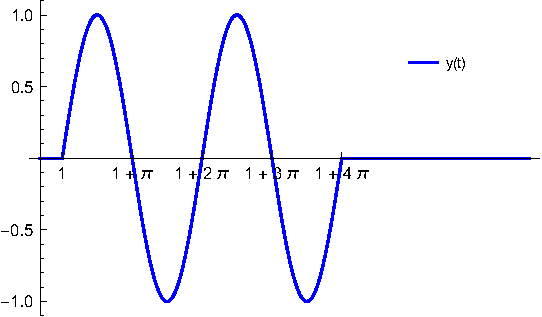
\includegraphics[width=8.5cm]{images/Double_Dirac_SHM.pdf}}
}
\slide{
The convolution theorem also allows us to solve integro-differential equations. \ex{$y'(t)=e^t+2\intop_0^ty(t-\tau)e^\tau d\tau\quad\text{with}\quad y(0)=0$}

\student{\algn{sY(s) =\frac{1}{s-1} +&2 \lap{\intop_0^ty(t-\tau)e^\tau d\tau} = \frac{1}{s-1} +2 Y(s) \frac{1}{s-1}\\
\left(s-\frac{2}{s-1}\right) Y(s) &= \frac{1}{s-1} \qquad \Rightarrow \qquad
\frac{\overbrace{s^2-s-2}^{(s-2)(s+1)}}{\cancel{s-1}} Y(s) = \frac{1}{\cancel{s-1}}\\
Y(s)&=\frac{1}{(s-2)(s+1)}}}
\settoggle{covered}{false}
\student{
\algn{
y(t)&=\intop_0^te^{2\tau} e^{-(t-\tau)}d\tau  = e^{-t} \intop_0^t e^{3\tau} d\tau=\frac{e^{-t}}{3}\left[ e^{3\tau}\right]_{\tau=0}^t\\
&=\frac13\left(e^{2t}-e^{-t}\right)
}
}
}
\settoggle{covered}{false}
\slide[Convolution Theorem: Special Case]{
Let $f(t)$ be an integrable function and $g(t)=1$.
\algn{\lap{f(t)\ast g(t)}&=F(s)G(s)\\
\lap{\intop_0^t f(\tau) d\tau}&=\student{F(s)\lap{1}}\\
&\student{=\frac{F(s)}{s} \qquad \text{or}\qquad \lapinv{\frac{F(s)}{s}} =\intop_0^t f(\tau) d\tau }
}\ex{Find the inverse Laplace tranforms of $H(s)=\frac{1}{s(s+7)}$}
\student{\algn{h(t)&=\intop_0^t e^{-7\tau} d\tau=-\frac17\left[ e^{-7\tau}\right]_{\tau=0}^t = -\frac17 \left( e^{-7t} -1 \right)}}
}
\end{document}